\section{Forging Optimization Control}
\label{sec:control}

This section builds a continuous speed-profile policy on top of the world model in Section \ref{sec:world_model}. With the world model as a propagatable environment, the policy performs stepwise decision-making conditioned on the latent state inside the world model to generate the entire continuous speed profile, which is then deployed to the equipment once; training is conducted entirely within the world model without interacting with the real equipment. The overall pipeline is shown in Fig.~\ref{fig:control}.

\begin{figure}[htbp]
\centerline{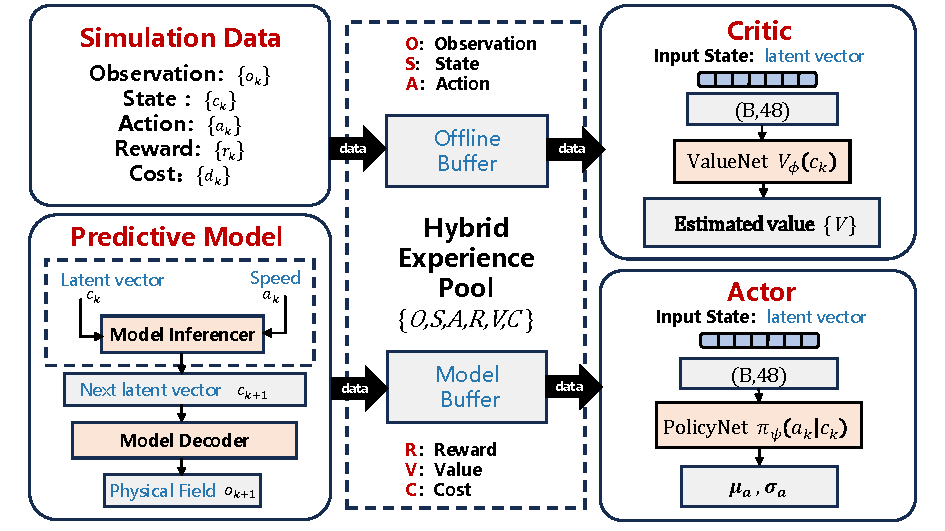
\includegraphics[width=12cm]{control-1-wide.pdf}}
\caption{Schematic of policy training.}
\label{fig:control}
\end{figure}

\subsection{Decision Problem Formulation within the World Model}
The die-speed decision is formulated as a finite-horizon constrained Markov decision process (CMDP) with safety constraints~\cite{altman2021constrained}. This process is defined only within the world model and is used for offline policy training: the state transition is provided by the world model, and the entire training does not interact with the equipment; after training, the complete speed profile is deployed once and executed. The process is defined by five elements---state, action, transition, reward, and cost---and the objective is to maximize the cumulative reward subject to the cumulative cost constraints. Each element is defined below.

\textbf{State.} The latent state $c_k\in\mathbb{R}^{d}$ inside the world model serves as the state, and both the policy and the value function take the latent state $c_k$ as input. The decoded geometry--multi-physics point cloud (i.e., the reconstructed point cloud $\hat{X}_k$ in Section \ref{sec:world_model}) $o_k=\mathrm{Dec}(c_k)\in\mathbb{R}^{N\times 6}$ ($o_k$ is a deterministic function of $c_k$) is used only to compute the reward and cost during training and does not participate in decision-making.

\textbf{Action.} The policy determines the die speed step by step along the stroke: at step $k$, at the cumulative stroke (displacement) $s_k$, it outputs the speed of that step $v_k=a_k\in\mathbb{R}$, bounded by the equipment capability, $v_k\in[v_{\min},v_{\max}]$. The per-step speeds constitute the speed profile $v(s)$ with the stroke as the independent variable; then, via $dt=ds/v(s)$, the independent variable is converted from displacement $s$ to time $t$, yielding the speed profile with time as the independent variable
\begin{equation}
v_y(t)=v\big(s(t)\big),
\end{equation}
where $s(t)$ is the cumulative stroke as a function of time, obtained by integrating the above and monotonically increasing. This profile $v_y(t)$ is the speed--time command directly executable by the press and the reference for efficiency metrics such as forging time.

\textbf{Transition.} $c_{k+1}=c_k+\int_{s_k}^{s_{k+1}}g\big(c,v_y(t)\big)\,ds$: the latent state is propagated by integrating along the stroke over the $k$-th stroke segment $[s_k,s_{k+1}]$ according to $v(s)$.

\textbf{Stroke constraint.} The total stroke satisfies
\begin{equation}
\int_{0}^{t_f}v_y(t)\,dt=\Delta h .
\end{equation}
The duration of each segment is determined by the speed of that step, $\Delta t_k=\int_{s_k}^{s_{k+1}}ds/v(s)$: the higher the speed, the shorter the segment duration.

\textbf{Reward.} The reward balances efficiency and quality step by step. At step $k$, the world model decodes the stress field $\{\hat{\sigma}_i\}_{i=1}^{N}$, which is sorted in descending order, with the top $m$ values denoted $\hat{\sigma}_{(1)}\ge\hat{\sigma}_{(2)}\ge\cdots\ge\hat{\sigma}_{(m)}$. Then define
\begin{equation}
\bar{\sigma}_k=\frac{1}{m}\sum_{j=1}^{m}\hat{\sigma}_{(j)},\qquad
u_k=\frac{\mathrm{std}(\hat{\sigma}_i)}{\mathrm{mean}(\hat{\sigma}_i)},
\end{equation}
where $\bar{\sigma}_k$ characterizes the magnitude of the field stress level, and $u_k$ is the coefficient of variation of the stress field, characterizing the degree of stress concentration. The reward is defined as
\begin{equation}
r_k=w_1 e^{-\Delta t_k}-w_2\,\bar{\sigma}_k-w_3\,u_k,
\end{equation}
where $\Delta t_k$ is the duration of the $k$-th segment, and $w_1$, $w_2$, $w_3$ are weighting coefficients. The higher and more non-uniform the stress level, the faster the damage evolution; the reward penalizes these two terms, guiding the policy to shorten the forging time while keeping the workpiece in a low and uniform stress state, forming a complement between soft guidance and the hard damage constraint.

\textbf{Cost.} The cost characterizes the stepwise damage violation:
\begin{equation}
d_k=\mathrm{relu}(D_k-D_{\text{cr}}),
\end{equation}
where $D_k$ is the maximum accumulated damage of the workpiece at step $k$, i.e., the maximum of the damage field at that step, corresponding to the value of $D(t)$ in Eq.~\ref{equ:model} at step $k$; $D_{\text{cr}}$ is the critical damage value, and $d_k=0$ indicates no violation at that step.

\textbf{Optimization objective.} Maximize the cumulative reward while satisfying the damage constraint at every step:
\begin{equation}
\max_{\psi}\ \mathbb{E}\Big[\sum_{k}\gamma^{k} r_k\Big]\quad \text{s.t.}\quad \mathbb{E}[d_k]\le 0,\quad \forall k,
\end{equation}
where $\gamma$ is the discount factor. The constraint is stepwise, i.e., the accumulated damage must not exceed the critical value at every step ($D_k\le D_{\text{cr}}$).

\subsection{Continuous Representation of the Action}
The die speed is given continuously with the stroke as the independent variable and is differentiable along the stroke, so the speed profile $v_y(t)$ is smooth with no acceleration jumps and can be directly substituted into the stroke integral $\frac{dc}{ds}=g(c,\,v_y(t))$ of the latent dynamics model; the change of the single-step speed is thus smoothly distributed along the stroke without high-frequency jitter. The stroke equality holds automatically by the definition in the displacement domain, and the speed bounds and the damage constraint only delimit the feasible region without compressing the decision freedom.
% 【实验章待补：动作参数化消融——样条插值 vs 折线直连】

\subsection{Policy and Optimization Algorithm}
The policy is a Gaussian distribution conditioned on the latent state, outputting a normal distribution over the speed control at each step:
\begin{equation}
\begin{aligned}
\pi_{\psi}(a_k\mid c_k)&=\mathcal{N}\big(a_k;\ \mu_{\psi}(c_k),\ \sigma_{\psi}^{2}(c_k)\big),\\
a_k&=\mu_{\psi}(c_k)+\sigma_{\psi}(c_k)\odot\varepsilon,\quad \varepsilon\sim\mathcal{N}(0,I),
\end{aligned}
\end{equation}
where $\mu_{\psi}(c_k)\in\mathbb{R}$ and $\sigma_{\psi}(c_k)\in\mathbb{R}_{>0}$ are the mean and standard deviation output by the policy network $\pi_{\psi}:\mathbb{R}^{d}\to\mathbb{R}^{2}$, $\odot$ denotes element-wise multiplication, $a_k=v_k\in\mathbb{R}$ is the speed control at step $k$, and the variance is diagonal; at solving (inference) time the mean $\mu_{\psi}(c_k)$ is taken as the deterministic output (the policy network is a small MLP acting on the latent state).

Offline safe reinforcement learning is adopted to solve this CMDP: the stepwise constraint is converted into an unconstrained form via Lagrangian relaxation, defining a constraint-aware single-step reward
\begin{equation}
\tilde r_k=r_k-\lambda\,d_k,
\end{equation}
where $r_k$ is the reward at step $k$, $d_k$ is the damage violation at step $k$, and $\lambda$ is the dual variable. The Lagrangian function is constructed as
\begin{equation}
\mathcal{L}(\psi,\lambda)=\mathbb{E}\Big[\sum_{k}\gamma^{k}\ln \pi_{\psi}(a_k\mid c_k)\cdot A(c_k,a_k)\Big],
\end{equation}
where the stepwise advantage function is
\begin{equation}
A(c_k,a_k)=\tilde r_k+\gamma\hat{V}(c_{k+1})-\hat{V}(c_k),
\end{equation}
and $\hat{V}(c_k)$ is the value estimate (critic), whose network parameters are denoted $\phi$. The value network is trained by minimizing the one-step temporal-difference (TD) error, with the target side stopped-gradient:
\begin{equation}
\mathcal{L}_{V}(\phi)=\mathbb{E}\Big[\big(\hat{V}(c_k)-\big[\tilde r_k+\gamma\,\mathrm{sg}(\hat{V}(c_{k+1}))\big]\big)^{2}\Big],
\end{equation}
where $\mathrm{sg}(\cdot)$ is the stop-gradient operator. To encourage exploration and prevent premature convergence, a stepwise entropy regularization term is added. Furthermore, the ``slow-then-fast'' shape of the die speed has a clear motivation for damage control~\cite{bambach2018towards}: at the early stage of deformation the contact impact and local stress concentration make damage initiation most sensitive, so a low speed suppresses damage accumulation, and after the material softens sufficiently the speed is increased to shorten the high-temperature dwell. This work does not follow that prior work in hard-coding the prior into a parameterized curve family; instead, it is reduced to a soft preference via a monotonicity regularization term:
\begin{equation}
\mathcal{R}_{\text{mono}}(\psi)=\mathbb{E}\Big[\sum_{k}\gamma^{k}\,\max\big(0,\,v_k-v_{k+1}\big)\Big],
\end{equation}
This regularization is positive only when $v_k>v_{k+1}$ (the current step is faster than the next, i.e., decelerating) and zero otherwise, so it penalizes only the deceleration segments and induces a monotonically non-decreasing speed; it has no preference over the acceleration magnitude and thus does not restrict the policy's ability to represent any speed profile. Incorporating the entropy regularization and the monotonicity regularization into the objective yields
\begin{equation}
\begin{aligned}
\mathcal{J}(\psi,\lambda)=&\,\mathcal{L}(\psi,\lambda)+\eta\,\mathbb{E}\Big[\sum_{k}\gamma^{k}H\big[\pi_{\psi}(\cdot\mid c_k)\big]\Big]\\
&-\lambda_m\,\mathcal{R}_{\text{mono}}(\psi),
\end{aligned}
\end{equation}
where $\eta$ and $\lambda_m$ are the entropy coefficient and the monotonicity regularization strength, respectively, and $H[\cdot]$ is the policy entropy.

The optimization adopts dual gradient ascent: first fix $\lambda$ and maximize $\mathcal{J}$ with respect to $\psi$ to update the policy parameters; then fix $\psi$ and update the dual variable according to the degree of constraint violation
\begin{equation}
\lambda\leftarrow\max\big(0,\ \lambda+\alpha_{\lambda}\bar{d}\big),\qquad \bar{d}=\max_{k}\,(D_k-D_{\text{cr}}),
\end{equation}
where $\alpha_{\lambda}$ is the dual step size, and $\bar{d}$ is the maximum (signed) difference between the damage and the critical value over all steps along the entire trajectory. When a violation step exists ($\bar{d}>0$), $\lambda$ increases to strengthen the penalty; when every step is below the critical value ($\bar{d}<0$), $\lambda$ decreases to relax the constraint. The policy training collects experience via closed-loop rollout within the world model: at each step the speed $v_k$ is output conditioned on the latent state $c_k$, and the state is advanced autoregressively by the world model as $c_{k+1}=c_k+\int_{s_k}^{s_{k+1}}g(c,v_y(t))\,ds$, isomorphic to the solving stage; the whole process is offline and requires no interaction with the real equipment. Training uses a mixed experience replay buffer, where the transition samples come from the finite-element simulation dataset $\mathcal{B}$ and the data generated by world-model propagation; $\rho$ is the proportion of simulation data in a batch, and the two kinds of samples are mixed according to this proportion to jointly participate in the update.

\subsection{Decision Solving and Execution}
In the solving stage, the policy performs stepwise rollout decision-making within the world model: at step $k$, the speed $v_k$ is output conditioned on the latent state $c_k$; after obtaining the per-step speeds, the entire profile $v_y(t)$ is assembled. In the execution stage, this profile is deployed to the equipment once, and the equipment provides no online feedback. Compared with the single-shot parametric policy that outputs $\theta$ once and generates the entire profile in a feedforward manner, the stepwise decision-making of this work can exploit the evolution information of damage, stress, and other quantities step by step and adapt to different initial temperature fields.
